\section{Operação do \textit{tracking}}

Como mostrado na \textbf{figura \ref{fig:GNSS_flow_graph}}, ao final de todo o processamento que ocorre dentro de um receptor de sinais GNSS, o que se deseja é obter posição, velocidade e tempo (PVT). E para tal, não diferentemente de toda análise física para determinação de posição, velocidade e tempo, incialmente adota-se um referencial, que, no caso de navegação por satélite, será o próprio satélite.

Porém, não basta um satélite apenas, pois isso não expressaria com exatidão alguma a posição do receptor em relação ao satélite. Se o satélite estivesse no centro de uma circunferência e o receptor na borda dessa, de modo que se pudesse argumentar que a distância entre a o satélite o receptor seja de $r$, o raio dessa circunferência, o receptor poderia estar em qualquer ponto dessa circunferêcia, em qualquer posição dos 360º disponíveis e a distância continuaria sendo a mesma sem que se pudesse de fato determinar a posição do receptor.

Para resolver esse probelama, usa-se uma técnica conhecida como trilateração, que está representada a seguir na \textbf{figura \ref{fig:Trilateração}}. Agora, em vez de existirem várias posições possíveis para que o receptor ocupe em relação ao satélite, existe apenas uma possível, que está na intersecção da transmissão feita pelos três satélites. 

\begin{figure}[ht]
    \centering
    \caption{Representação bidimensional da trialteração ideal}
    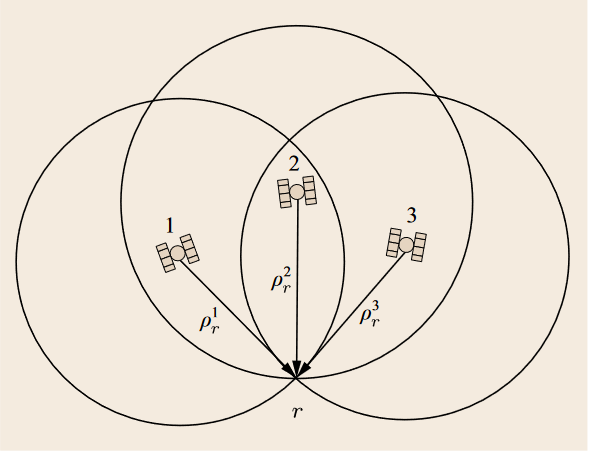
\includegraphics[width = 0.6 \textwidth]{figuras/Trilateração.png}

    Fonte: \cite{Teunissen2017}
    \label{fig:Trilateração}
\end{figure}

Apesar de a \textbf{figura \ref{fig:Trilateração}} mostrar um caso bidimensional, o probelma real ocorre em um caso tridimensional, o que torna o campo de alcance dos sinais dos satélites não mais em circunferências, mas esferas, sendo que o ponto estimado do receptor estará na intersecção das 3 esferas de sinal enviada por eles. E sua posição em relação a eles pode ser determinada por:

\begin{equation}
    \rho_{r1} =\sqrt{(x_r-x_1)^2+(y_r-y_1)^2+(z_r-z_1)^2}
\end{equation}
\begin{equation}
    \rho_{r2} =\sqrt{(x_r-x_2)^2+(y_r-y_2)^2+(z_r-z_2)^2}
\end{equation}
\begin{equation}
    \rho_{r3} =\sqrt{(x_r-x_3)^2+(y_r-y_3)^2+(z_r-z_3)^2}
\end{equation}
,onde $\rho_{rn}$ é a distância do receptor para o satélite n.

Por mais que esse modelo já esteja levando em conta fatores como posicionamento em três dimensões, ainda há algumas simplificações que estão implicitas nele e que podem levar a grandes erros. Uma dessas é não considerar o tempo de propagação do sinal desde o satélite emissor ao receptor.

Por mais que a velocidade da luz seja muito alta, a propagação de uma onda eletromagnética através do espaço não acontece instantaneamente, ou seja, leva-se um tempo para que o sinal enviado do satélite chegue ao receptor. E é justamente por meio desse atraso, $\tau$, que é medida a distância que o satelite está do receptor. 

Para fazer essa estimativa de tempo, o receptor faz uso de um oscilador interno, como mostra a \textbf{figura \ref{fig:GNSS_components}}, que busca reproduzir um tipo específico do sinal que é enviado pelo satélite, como é mostrado na \textbf{figura \ref{fig:Recepção_GNSS}}. Como explica \cite{Teunissen2017}, esse sinal que é gerado localmente é continuamente comparado ao sinal que está chegando na entrada. Para que esse sinal seja semelhante ao que está chegando, é necessário que haja sincronismo entre o clock que está produzindo a replica e o que gerou o sinal com que é comparado. Com essa defasagem que está sendo colocada no sinal gerado, é possível obter a distância que o receptor está do satélite.


\begin{figure}[ht]
    \centering
    \caption{Recepção e geração de réplica do sinal de GNSS}
    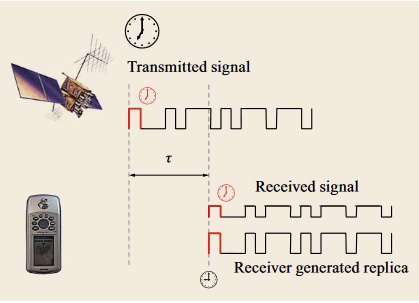
\includegraphics[width = 0.6\textwidth]{figuras/Recepção do sinal de GNSS.png}

    Fonte: \cite{Teunissen2017}
    \label{fig:Recepção_GNSS}
\end{figure}


Todavia, quando se está tratando de velocidades tão altas como as da luz, pequenos erros de tempo transformam-se em grandes erros de distância e a capacidade de sincronizar o clock do oscilador local com o do transmissor torna-se um fator determinante para a posição do receptor do sinal, inserindo uma incerteza de posição na trilaterção representada na \textbf{figura \ref{fig:Trilateração}}. Condensando o problema para 2 dimensões, a incerteza inserida seria como apresentado na \textbf{figura \ref{fig:Trilateração real}}. Nela é possível ver que a posição precisa da trilateração será tão mais precisa quanto menor for o raio da circunfeência tangente àquelas que representam o sinal emitido pelos satélites. Essa circunferência mais interna é exatamente o erro de posicionamento que será causado pelo dessincronismo entre os sinais.

Como várias informações a respieto do PVT são retiradas não apenas do conteúdo da mensagem, mas também de seu formato, os sinais de GNSS possuem algumas epecificidades que permitem a obtenção dessas informações. Agora, esses serão vistos em mais detalhes. 

\begin{figure}[h]
    \centering
    \caption{Trilateração com a incerteza associada à dessincronia do clock do receptor em relação ao do transmissor, $\Delta_Q$}
    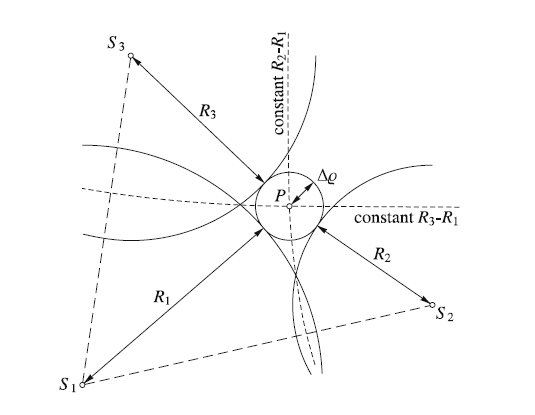
\includegraphics[width = 0.6 \textwidth]{figuras/Trilateração real.png}
    
    Fonte: \cite{Wellenhoff2008}
    \label{fig:Trilateração real}
\end{figure}

\subsection{O sinal GNSS}